% Options for packages loaded elsewhere
\PassOptionsToPackage{unicode}{hyperref}
\PassOptionsToPackage{hyphens}{url}
%
\documentclass[
]{article}
\usepackage{amsmath,amssymb}
\usepackage{iftex}
\ifPDFTeX
  \usepackage[T1]{fontenc}
  \usepackage[utf8]{inputenc}
  \usepackage{textcomp} % provide euro and other symbols
\else % if luatex or xetex
  \usepackage{unicode-math} % this also loads fontspec
  \defaultfontfeatures{Scale=MatchLowercase}
  \defaultfontfeatures[\rmfamily]{Ligatures=TeX,Scale=1}
\fi
\usepackage{lmodern}
\ifPDFTeX\else
  % xetex/luatex font selection
\fi
% Use upquote if available, for straight quotes in verbatim environments
\IfFileExists{upquote.sty}{\usepackage{upquote}}{}
\IfFileExists{microtype.sty}{% use microtype if available
  \usepackage[]{microtype}
  \UseMicrotypeSet[protrusion]{basicmath} % disable protrusion for tt fonts
}{}
\makeatletter
\@ifundefined{KOMAClassName}{% if non-KOMA class
  \IfFileExists{parskip.sty}{%
    \usepackage{parskip}
  }{% else
    \setlength{\parindent}{0pt}
    \setlength{\parskip}{6pt plus 2pt minus 1pt}}
}{% if KOMA class
  \KOMAoptions{parskip=half}}
\makeatother
\usepackage{xcolor}
\usepackage[margin=1in]{geometry}
\usepackage{color}
\usepackage{fancyvrb}
\newcommand{\VerbBar}{|}
\newcommand{\VERB}{\Verb[commandchars=\\\{\}]}
\DefineVerbatimEnvironment{Highlighting}{Verbatim}{commandchars=\\\{\}}
% Add ',fontsize=\small' for more characters per line
\usepackage{framed}
\definecolor{shadecolor}{RGB}{248,248,248}
\newenvironment{Shaded}{\begin{snugshade}}{\end{snugshade}}
\newcommand{\AlertTok}[1]{\textcolor[rgb]{0.94,0.16,0.16}{#1}}
\newcommand{\AnnotationTok}[1]{\textcolor[rgb]{0.56,0.35,0.01}{\textbf{\textit{#1}}}}
\newcommand{\AttributeTok}[1]{\textcolor[rgb]{0.13,0.29,0.53}{#1}}
\newcommand{\BaseNTok}[1]{\textcolor[rgb]{0.00,0.00,0.81}{#1}}
\newcommand{\BuiltInTok}[1]{#1}
\newcommand{\CharTok}[1]{\textcolor[rgb]{0.31,0.60,0.02}{#1}}
\newcommand{\CommentTok}[1]{\textcolor[rgb]{0.56,0.35,0.01}{\textit{#1}}}
\newcommand{\CommentVarTok}[1]{\textcolor[rgb]{0.56,0.35,0.01}{\textbf{\textit{#1}}}}
\newcommand{\ConstantTok}[1]{\textcolor[rgb]{0.56,0.35,0.01}{#1}}
\newcommand{\ControlFlowTok}[1]{\textcolor[rgb]{0.13,0.29,0.53}{\textbf{#1}}}
\newcommand{\DataTypeTok}[1]{\textcolor[rgb]{0.13,0.29,0.53}{#1}}
\newcommand{\DecValTok}[1]{\textcolor[rgb]{0.00,0.00,0.81}{#1}}
\newcommand{\DocumentationTok}[1]{\textcolor[rgb]{0.56,0.35,0.01}{\textbf{\textit{#1}}}}
\newcommand{\ErrorTok}[1]{\textcolor[rgb]{0.64,0.00,0.00}{\textbf{#1}}}
\newcommand{\ExtensionTok}[1]{#1}
\newcommand{\FloatTok}[1]{\textcolor[rgb]{0.00,0.00,0.81}{#1}}
\newcommand{\FunctionTok}[1]{\textcolor[rgb]{0.13,0.29,0.53}{\textbf{#1}}}
\newcommand{\ImportTok}[1]{#1}
\newcommand{\InformationTok}[1]{\textcolor[rgb]{0.56,0.35,0.01}{\textbf{\textit{#1}}}}
\newcommand{\KeywordTok}[1]{\textcolor[rgb]{0.13,0.29,0.53}{\textbf{#1}}}
\newcommand{\NormalTok}[1]{#1}
\newcommand{\OperatorTok}[1]{\textcolor[rgb]{0.81,0.36,0.00}{\textbf{#1}}}
\newcommand{\OtherTok}[1]{\textcolor[rgb]{0.56,0.35,0.01}{#1}}
\newcommand{\PreprocessorTok}[1]{\textcolor[rgb]{0.56,0.35,0.01}{\textit{#1}}}
\newcommand{\RegionMarkerTok}[1]{#1}
\newcommand{\SpecialCharTok}[1]{\textcolor[rgb]{0.81,0.36,0.00}{\textbf{#1}}}
\newcommand{\SpecialStringTok}[1]{\textcolor[rgb]{0.31,0.60,0.02}{#1}}
\newcommand{\StringTok}[1]{\textcolor[rgb]{0.31,0.60,0.02}{#1}}
\newcommand{\VariableTok}[1]{\textcolor[rgb]{0.00,0.00,0.00}{#1}}
\newcommand{\VerbatimStringTok}[1]{\textcolor[rgb]{0.31,0.60,0.02}{#1}}
\newcommand{\WarningTok}[1]{\textcolor[rgb]{0.56,0.35,0.01}{\textbf{\textit{#1}}}}
\usepackage{graphicx}
\makeatletter
\def\maxwidth{\ifdim\Gin@nat@width>\linewidth\linewidth\else\Gin@nat@width\fi}
\def\maxheight{\ifdim\Gin@nat@height>\textheight\textheight\else\Gin@nat@height\fi}
\makeatother
% Scale images if necessary, so that they will not overflow the page
% margins by default, and it is still possible to overwrite the defaults
% using explicit options in \includegraphics[width, height, ...]{}
\setkeys{Gin}{width=\maxwidth,height=\maxheight,keepaspectratio}
% Set default figure placement to htbp
\makeatletter
\def\fps@figure{htbp}
\makeatother
\setlength{\emergencystretch}{3em} % prevent overfull lines
\providecommand{\tightlist}{%
  \setlength{\itemsep}{0pt}\setlength{\parskip}{0pt}}
\setcounter{secnumdepth}{-\maxdimen} % remove section numbering
\usepackage{booktabs}
\usepackage{longtable}
\usepackage{array}
\usepackage{multirow}
\usepackage{wrapfig}
\usepackage{float}
\usepackage{colortbl}
\usepackage{pdflscape}
\usepackage{tabu}
\usepackage{threeparttable}
\usepackage{threeparttablex}
\usepackage[normalem]{ulem}
\usepackage{makecell}
\usepackage{xcolor}
\ifLuaTeX
  \usepackage{selnolig}  % disable illegal ligatures
\fi
\IfFileExists{bookmark.sty}{\usepackage{bookmark}}{\usepackage{hyperref}}
\IfFileExists{xurl.sty}{\usepackage{xurl}}{} % add URL line breaks if available
\urlstyle{same}
\hypersetup{
  pdftitle={NYC RealEstate},
  pdfauthor={Fredrick Jones, Jian Quan Chen, Tilon Bobb},
  hidelinks,
  pdfcreator={LaTeX via pandoc}}

\title{NYC RealEstate}
\author{Fredrick Jones, Jian Quan Chen, Tilon Bobb}
\date{2024-04-24}

\begin{document}
\maketitle

{
\setcounter{tocdepth}{2}
\tableofcontents
}
\begin{Shaded}
\begin{Highlighting}[]
\CommentTok{\#Clear all}
\FunctionTok{rm}\NormalTok{(}\AttributeTok{list =} \FunctionTok{ls}\NormalTok{())}

\FunctionTok{options}\NormalTok{(}\AttributeTok{scipen =} \DecValTok{999}\NormalTok{)}
\end{Highlighting}
\end{Shaded}

\hypertarget{abstract}{%
\subsection{Abstract}\label{abstract}}

This study uses real estate transaction data to investigate the factors
influencing property values in New York City. The dataset includes a
variety of parameters that were gathered from public records and real
estate listings, including property location, kind, size, and sale
price. To understand the distribution and interrelationships of the
dataset, exploratory data analysis (EDA) is the first systematic stage
in the study technique. Data preparation is a step that comes next in
order to encode categorical variables, handle missing values, and create
new features. Stepwise regression, generalized linear models (GLM),
robust regression, and conventional linear regression are all included
in the design of regression models. The goal of developing predictive
models that offer robustness against outliers while generalizing
effectively to new data is achieved through the use of goodness-of-fit
measures and diagnostic tests for residual analysis as the basis for
model selection.

\hypertarget{keywords}{%
\subsection{Keywords}\label{keywords}}

NYC Real Estate Data Analysis Regression Modeling Housing Market Trends
Neighborhood Analysis

\hypertarget{introduction}{%
\subsection{Introduction}\label{introduction}}

The New York real estate market is one of the most dynamic and
influential sectors of urban development. With every real estate
transaction representing a tangible real estate exchange, the NYC real
estate market is a barometer of the city's socioeconomic landscape. In
this report, we take an in-depth look at the NYC market through insights
from a diverse dataset of New York real estate sales records.

\hypertarget{background-and-motivation}{%
\subsubsection{Background and
Motivation}\label{background-and-motivation}}

The database under study contains a wealth of data spanning two decades,
providing a detailed chronicle of real estate transactions in the five
boroughs of New York - Manhattan, the Bronx, Brooklyn, Queens and Staten
Island. Our analysis is based on the foundation created by this dataset,
which provides insight into the multifaceted dynamics of NYC real estate
sales.

The motivation is to identify the factors that influence NYC real estate
prices, so our research is based on a variety of analytical techniques.
and methods. From data analysis to regression modeling, we seek to
uncover the complex interplay of variables that affect real estate. By
examining real estate sales trends, identifying key predictors of sales
prices, and assessing the impact of factors such as property size,
location, and tax bracket, we aim to shed light on the mechanics behind
the NYC real estate world.

As we delve into the depths of the NYC real estate market, our analysis
aims to provide stakeholders with actionable insights on investors and
from decision makers to real estate developers and potential buyers. By
uncovering the drivers of real estate prices and delineating market
trends, we aim to provide decision makers with the information they need
to navigate the complexities of the real estate ecosystem.

\hypertarget{literature-review}{%
\subsection{Literature Review}\label{literature-review}}

\hypertarget{michael-gaynors-project}{%
\paragraph{\texorpdfstring{\href{https://medium.com/@mgaynor228/analysis-of-nyc-property-sales-9af7686aa2ca}{Michael
Gaynor's
Project}}{Michael Gaynor's Project}}\label{michael-gaynors-project}}

Michael Gaynor conducted a project to explore the NYC real estate market
using SQL queries and Tableau visualization techniques. His
investigation aimed to answer four main questions:

\begin{enumerate}
\def\labelenumi{\arabic{enumi}.}
\tightlist
\item
  Which of the five boroughs is the most expensive?
\item
  Which of the five boroughs have the most sales?
\item
  What type of properties sell the most in each of the 5 boroughs?
\item
  What property type influences sales?
\end{enumerate}

Gaynor's approach involved understanding the task, prepping the data,
analyzing the data using SQL queries and Tableau visualization, and
presenting the findings through an interactive dashboard. Through his
analysis, Gaynor discovered insights such as the most expensive borough,
the borough with the most property sales, and the types of properties
that sell the most in each borough.

\hypertarget{comparison-and-evaluation}{%
\subsubsection{Comparison and
Evaluation}\label{comparison-and-evaluation}}

Gaynor's research utilized the same NYC real estate dataset to address
similar questions as our investigation. However, there are significant
differences between Gaynor's approach and our own project:

\begin{itemize}
\item
  \textbf{Methodology}: Gaynor primarily used SQL queries and Tableau
  visualization tools for data analysis, while our investigation
  utilized R programming language. Our approach involved a combination
  of data preprocessing, exploratory data analysis (EDA), statistical
  modeling, and visualization techniques implemented in R.
\item
  \textbf{Presentation of Findings}: Gaynor's project focused on
  presenting the results through an interactive dashboard created in
  Tableau. In contrast, our investigation may present the findings
  through various formats such as tables, charts, and narratives within
  the R Markdown document.
\item
  \textbf{Data Preprocessing}: While Gaynor mentioned data cleaning and
  preprocessing, the details of these steps were not extensively
  discussed. In our investigation, we employed specific techniques such
  as handling missing values, outlier detection and removal, and data
  transformation using R packages like dplyr and tidyr.
\item
  \textbf{Statistical Modeling}: Our investigation may involve the
  application of statistical models such as linear regression,
  generalized linear models, or machine learning algorithms to explore
  relationships between variables and predict real estate prices.
  Gaynor's project did not explicitly mention the use of statistical
  modeling.
\end{itemize}

\hypertarget{advantages-and-drawbacks}{%
\subsubsection{Advantages and
Drawbacks}\label{advantages-and-drawbacks}}

The advantages of Gaynor's approach include:

\begin{itemize}
\tightlist
\item
  Comprehensive analysis of the NYC real estate market using SQL and
  Tableau.
\item
  Clear presentation of findings through interactive visualization.
\end{itemize}

However, there may be some drawbacks to Gaynor's approach, such as:

\begin{itemize}
\tightlist
\item
  Reliance on SQL and Tableau tools may limit accessibility for
  researchers unfamiliar with these technologies.
\item
  Lack of detailed explanation of data cleaning and preprocessing steps.
\end{itemize}

\hypertarget{regression-modeling-methodology}{%
\subsection{Regression Modeling
Methodology}\label{regression-modeling-methodology}}

\hypertarget{data-preparation}{%
\subsubsection{Data Preparation}\label{data-preparation}}

The first part of our analysis consisted of importing the dataset that
included data on property sales in New York City. After we uploaded the
dataset, we conducted an exploratory data analysis to understand its
organization, factors, and any problems that required attention.

During the exploratory data analysis, we faced one of the first hurdles
with the discovery of missing values in multiple columns. To tackle this
problem, we methodically pinpointed the variables with incomplete data
and assessed the percentage of missing values in each instance. After
careful deliberation, we made the choice to eliminate data points
containing incomplete information, as they comprised less than 5\% of
the entire data set. This method enabled us to keep a large part of the
data while reducing the effect of missing values on future analyses.

After addressing missing data, we focused on the distribution of
numerical variables in the dataset. We noticed that many variables
showed noticeable skewness, suggesting possible departures from normal
distribution. To tackle this problem, we utilized Tukey's method for
identifying and eliminating outliers. Our goal was to enhance the
robustness of future analyses by improving the distributional properties
of numeric variables through the identification and exclusion of
outliers from the dataset.

Additionally, we examined the connections between variables using
correlation analysis. This included computing correlation coefficients
for pairs of numerical variables in order to evaluate the magnitude and
orientation of their relationships. During this examination, we found
multiple variables that showed strong positive relationships with each
other, along with variables that had weaker or negative relationships.
These results offered valuable information on potential factors that
could predict real estate prices and guided the choice of variables for
inclusion in regression analysis.

In addition, we analysed changes over time by graphing the time-based
pattern of property values in New York City. This examination showed a
rising pattern in mean sale prices over time, with variations in certain
time frames. Through the visualization of time-based trends, we achieved
a better comprehension of the fluctuations within the real estate market
of New York City, pinpointing potential influences on property price
fluctuations.

\hypertarget{regression-modelling}{%
\subsubsection{Regression Modelling}\label{regression-modelling}}

After completing thorough data preparation and exploratory analysis, we
focused on the main objective of our research: using regression
modelling to forecast real estate prices in New York City. The method we
used involved carefully building linear regression models, using
different predictor variables to understand the complex factors
influencing real estate prices. Leading our regression modelling was the
incorporation of important predictor variables that were considered to
have a significant impact on real estate prices. These variables
included a wide range of factors, each providing valuable perspectives
on the intricate fabric of the New York City real estate market.
Included in these predictors were the quantity of housing units in a
property, offering an insight into its size and ability to house
residents. The categorization of taxes for properties at various points
highlighted their financial status and legal ramifications, revealing
insights into the larger economic and legal environments in which these
properties function.

Furthermore, the year in which the building was constructed was
identified as a crucial factor in predicting real estate values, giving
a historical perspective on how they change over time. We aimed to
capture temporal trends and identify any seasonal or cyclical patterns
that could affect pricing dynamics by including the sale date of
properties in our models. Moreover, factors like total area and land
area were essential in evaluating the physical size and spatial
characteristics of properties, enhancing our comprehension of their
inherent value.

By conducting thorough regression analysis, we discovered significant
statistical connections between these predictor variables and property
prices, revealing the complex interaction of factors that influence
pricing decisions in the real estate market of New York City.
Nevertheless, even though our models were strong, the adjusted R-squared
values suggested that there might be additional variability that was not
accounted for, indicating the presence of hidden factors that were not
included in our analysis.

\hypertarget{explorartory-data-analysis}{%
\subsection{Explorartory Data
Analysis}\label{explorartory-data-analysis}}

\hypertarget{loading-data}{%
\subsubsection{Loading Data}\label{loading-data}}

\begin{Shaded}
\begin{Highlighting}[]
\NormalTok{nyc\_data }\OtherTok{\textless{}{-}} \FunctionTok{read.csv}\NormalTok{(}\StringTok{"C:/Users/Jian/Desktop/DATA 621 {-}Business Analytics and Data Mining/Final Project/nyc{-}property{-}sales.csv"}\NormalTok{)}

\CommentTok{\#head(nyc\_data)}
\end{Highlighting}
\end{Shaded}

\hypertarget{glipmse-of-the-dataset}{%
\paragraph{Glipmse of the dataset}\label{glipmse-of-the-dataset}}

\begin{Shaded}
\begin{Highlighting}[]
\FunctionTok{glimpse}\NormalTok{(nyc\_data)}
\end{Highlighting}
\end{Shaded}

\begin{verbatim}
## Rows: 1,603,826
## Columns: 21
## $ BOROUGH                        <int> 1, 1, 1, 1, 1, 1, 1, 1, 1, 1, 1, 1, 1, ~
## $ NEIGHBORHOOD                   <chr> "ALPHABET CITY", "ALPHABET CITY", "ALPH~
## $ BUILDING.CLASS.CATEGORY        <chr> "01 ONE FAMILY DWELLINGS", "02 TWO FAMI~
## $ TAX.CLASS.AT.PRESENT           <chr> "1", "1", "2B", "2B", "2", "2A", "2A", ~
## $ BLOCK                          <int> 374, 377, 373, 373, 376, 377, 377, 379,~
## $ LOT                            <int> 46, 1, 16, 17, 54, 52, 52, 25, 45, 47, ~
## $ EASE.MENT                      <chr> "", "", "", "", "", "", "", "", "", "",~
## $ BUILDING.CLASS.AT.PRESENT      <chr> "A4", "S2", "C1", "C1", "C4", "C2", "C2~
## $ ADDRESS                        <chr> "347 EAST 4TH STREET", "110 AVENUE C", ~
## $ APARTMENT.NUMBER               <chr> "", "", "", "", "", "", "", "", "", "",~
## $ ZIP.CODE                       <dbl> 10009, 10009, 10009, 10009, 10009, 1000~
## $ RESIDENTIAL.UNITS              <dbl> 1, 2, 10, 10, 20, 5, 5, 7, 10, 10, 29, ~
## $ COMMERCIAL.UNITS               <dbl> 0, 1, 0, 0, 0, 0, 0, 1, 0, 0, 0, 1, 1, ~
## $ TOTAL.UNITS                    <dbl> 1, 3, 10, 10, 20, 5, 5, 8, 10, 10, 29, ~
## $ LAND.SQUARE.FEET               <dbl> 2116, 1502, 2204, 2204, 2302, 2168, 216~
## $ GROSS.SQUARE.FEET              <dbl> 4400, 2790, 8625, 8625, 9750, 3728, 372~
## $ YEAR.BUILT                     <dbl> 1900, 1901, 1899, 1900, 1900, 1900, 190~
## $ TAX.CLASS.AT.TIME.OF.SALE      <int> 1, 1, 2, 2, 2, 2, 2, 2, 2, 2, 2, 2, 2, ~
## $ BUILDING.CLASS.AT.TIME.OF.SALE <chr> "A4", "S2", "C1", "C1", "C4", "C2", "C2~
## $ SALE.PRICE                     <dbl> 399000, 2999999, 16800000, 16800000, 15~
## $ SALE.DATE                      <chr> "2022-09-29 00:00:00", "2022-09-15 00:0~
\end{verbatim}

Assessing missing values

\begin{Shaded}
\begin{Highlighting}[]
\CommentTok{\# Check for missing values}
\NormalTok{missing\_values }\OtherTok{\textless{}{-}} \FunctionTok{colSums}\NormalTok{(}\FunctionTok{is.na}\NormalTok{(nyc\_data))}

\CommentTok{\# View columns with missing values}
\NormalTok{missing\_columns }\OtherTok{\textless{}{-}} \FunctionTok{names}\NormalTok{(missing\_values[missing\_values }\SpecialCharTok{\textgreater{}} \DecValTok{0}\NormalTok{])}
\FunctionTok{print}\NormalTok{(missing\_columns)}
\end{Highlighting}
\end{Shaded}

\begin{verbatim}
## [1] "ZIP.CODE"                  "RESIDENTIAL.UNITS"        
## [3] "COMMERCIAL.UNITS"          "TOTAL.UNITS"              
## [5] "LAND.SQUARE.FEET"          "GROSS.SQUARE.FEET"        
## [7] "YEAR.BUILT"                "TAX.CLASS.AT.TIME.OF.SALE"
## [9] "SALE.PRICE"
\end{verbatim}

Drop missing values since there is less than 5\% of dataset missing
values hence safe to drop all missing values

\begin{Shaded}
\begin{Highlighting}[]
\NormalTok{clean\_nyc }\OtherTok{\textless{}{-}} \FunctionTok{na.omit}\NormalTok{(nyc\_data)}
\FunctionTok{str}\NormalTok{(clean\_nyc)}
\end{Highlighting}
\end{Shaded}

\begin{verbatim}
## 'data.frame':    1470283 obs. of  21 variables:
##  $ BOROUGH                       : int  1 1 1 1 1 1 1 1 1 1 ...
##  $ NEIGHBORHOOD                  : chr  "ALPHABET CITY" "ALPHABET CITY" "ALPHABET CITY" "ALPHABET CITY" ...
##  $ BUILDING.CLASS.CATEGORY       : chr  "01 ONE FAMILY DWELLINGS" "02 TWO FAMILY DWELLINGS" "07 RENTALS - WALKUP APARTMENTS" "07 RENTALS - WALKUP APARTMENTS" ...
##  $ TAX.CLASS.AT.PRESENT          : chr  "1" "1" "2B" "2B" ...
##  $ BLOCK                         : int  374 377 373 373 376 377 377 379 389 389 ...
##  $ LOT                           : int  46 1 16 17 54 52 52 25 45 47 ...
##  $ EASE.MENT                     : chr  "" "" "" "" ...
##  $ BUILDING.CLASS.AT.PRESENT     : chr  "A4" "S2" "C1" "C1" ...
##  $ ADDRESS                       : chr  "347 EAST 4TH STREET" "110 AVENUE C" "326 EAST 4TH STREET" "328 EAST 4TH STREET" ...
##  $ APARTMENT.NUMBER              : chr  "" "" "" "" ...
##  $ ZIP.CODE                      : num  10009 10009 10009 10009 10009 ...
##  $ RESIDENTIAL.UNITS             : num  1 2 10 10 20 5 5 7 10 10 ...
##  $ COMMERCIAL.UNITS              : num  0 1 0 0 0 0 0 1 0 0 ...
##  $ TOTAL.UNITS                   : num  1 3 10 10 20 5 5 8 10 10 ...
##  $ LAND.SQUARE.FEET              : num  2116 1502 2204 2204 2302 ...
##  $ GROSS.SQUARE.FEET             : num  4400 2790 8625 8625 9750 ...
##  $ YEAR.BUILT                    : num  1900 1901 1899 1900 1900 ...
##  $ TAX.CLASS.AT.TIME.OF.SALE     : int  1 1 2 2 2 2 2 2 2 2 ...
##  $ BUILDING.CLASS.AT.TIME.OF.SALE: chr  "A4" "S2" "C1" "C1" ...
##  $ SALE.PRICE                    : num  399000 2999999 16800000 16800000 158822 ...
##  $ SALE.DATE                     : chr  "2022-09-29 00:00:00" "2022-09-15 00:00:00" "2022-08-04 00:00:00" "2022-08-04 00:00:00" ...
##  - attr(*, "na.action")= 'omit' Named int [1:133543] 29 30 31 32 33 34 35 36 37 38 ...
##   ..- attr(*, "names")= chr [1:133543] "29" "30" "31" "32" ...
\end{verbatim}

All numeric variables are heavily skewed to the right, hence a clear
indication of outliers

All distributions exhibit a highly skewed pattern, with a single bar
extending vertically at the rightmost end of the x-axis, suggesting the
presence of potential outliers with extremely high unit counts.

\begin{Shaded}
\begin{Highlighting}[]
\CommentTok{\# Numeric variables}
\NormalTok{numeric\_vars }\OtherTok{\textless{}{-}} \FunctionTok{c}\NormalTok{(}\StringTok{"RESIDENTIAL.UNITS"}\NormalTok{, }\StringTok{"COMMERCIAL.UNITS"}\NormalTok{, }\StringTok{"TOTAL.UNITS"}\NormalTok{, }
                  \StringTok{"LAND.SQUARE.FEET"}\NormalTok{, }\StringTok{"GROSS.SQUARE.FEET"}\NormalTok{, }\StringTok{"SALE.PRICE"}\NormalTok{)}


\NormalTok{num\_data }\OtherTok{\textless{}{-}}\NormalTok{clean\_nyc[, numeric\_vars]}

\CommentTok{\# Set up the plot layout}
\FunctionTok{par}\NormalTok{(}\AttributeTok{mfrow =} \FunctionTok{c}\NormalTok{(}\DecValTok{2}\NormalTok{, }\DecValTok{3}\NormalTok{))}

\ControlFlowTok{for}\NormalTok{ (i }\ControlFlowTok{in} \DecValTok{1}\SpecialCharTok{:}\FunctionTok{length}\NormalTok{(}\FunctionTok{names}\NormalTok{(num\_data)))\{}
  \FunctionTok{print}\NormalTok{(i)}
  \FunctionTok{hist}\NormalTok{(num\_data[i], }\AttributeTok{main=}\StringTok{\textquotesingle{}hist\textquotesingle{}}\NormalTok{, }\AttributeTok{breaks=}\DecValTok{20}\NormalTok{, }\AttributeTok{prob=}\ConstantTok{TRUE}\NormalTok{)}
\NormalTok{\}}
\end{Highlighting}
\end{Shaded}

\begin{verbatim}
## [1] 1
\end{verbatim}

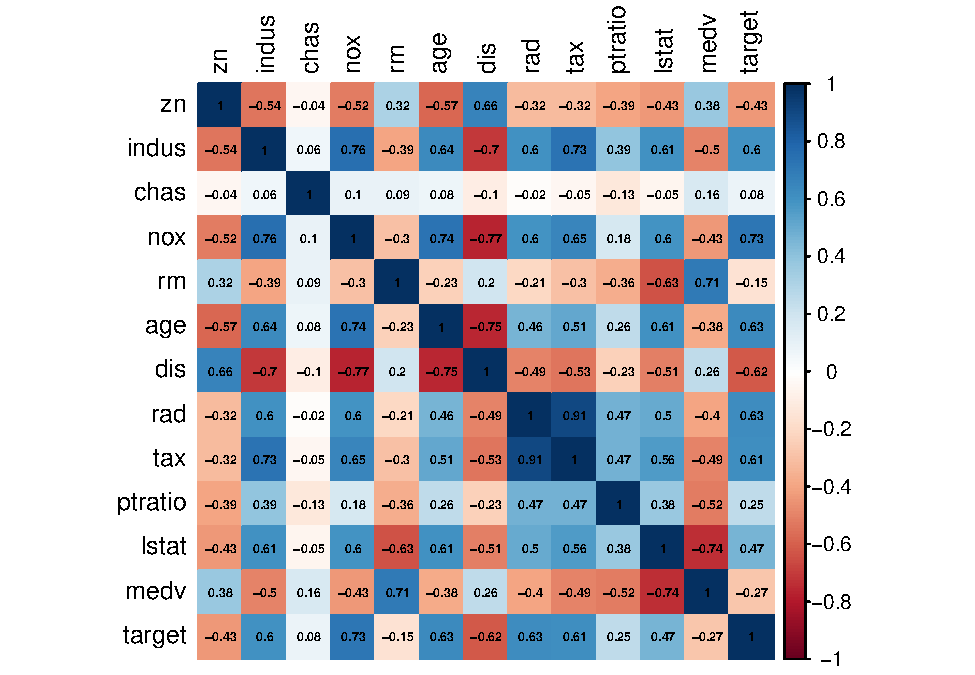
\includegraphics{NYCRealEstate_files/figure-latex/unnamed-chunk-6-1.pdf}

\begin{verbatim}
## [1] 2
\end{verbatim}

\includegraphics{NYCRealEstate_files/figure-latex/unnamed-chunk-6-2.pdf}

\begin{verbatim}
## [1] 3
\end{verbatim}

\includegraphics{NYCRealEstate_files/figure-latex/unnamed-chunk-6-3.pdf}

\begin{verbatim}
## [1] 4
\end{verbatim}

\includegraphics{NYCRealEstate_files/figure-latex/unnamed-chunk-6-4.pdf}

\begin{verbatim}
## [1] 5
\end{verbatim}

\includegraphics{NYCRealEstate_files/figure-latex/unnamed-chunk-6-5.pdf}

\begin{verbatim}
## [1] 6
\end{verbatim}

\includegraphics{NYCRealEstate_files/figure-latex/unnamed-chunk-6-6.pdf}

\begin{Shaded}
\begin{Highlighting}[]
\CommentTok{\# Reset the plot layout to default}
\FunctionTok{par}\NormalTok{(}\AttributeTok{mfrow =} \FunctionTok{c}\NormalTok{(}\DecValTok{2}\NormalTok{, }\DecValTok{3}\NormalTok{))}
\end{Highlighting}
\end{Shaded}

\begin{Shaded}
\begin{Highlighting}[]
\CommentTok{\# Function to remove outliers based on Tukey\textquotesingle{}s method}
\NormalTok{remove\_outliers }\OtherTok{\textless{}{-}} \ControlFlowTok{function}\NormalTok{(data, variable) \{}
\NormalTok{  q1 }\OtherTok{\textless{}{-}} \FunctionTok{quantile}\NormalTok{(data[[variable]], }\FloatTok{0.25}\NormalTok{)}
\NormalTok{  q3 }\OtherTok{\textless{}{-}} \FunctionTok{quantile}\NormalTok{(data[[variable]], }\FloatTok{0.75}\NormalTok{)}
\NormalTok{  iqr }\OtherTok{\textless{}{-}}\NormalTok{ q3 }\SpecialCharTok{{-}}\NormalTok{ q1}
\NormalTok{  lower\_bound }\OtherTok{\textless{}{-}}\NormalTok{ q1 }\SpecialCharTok{{-}} \FloatTok{1.5} \SpecialCharTok{*}\NormalTok{ iqr}
\NormalTok{  upper\_bound }\OtherTok{\textless{}{-}}\NormalTok{ q3 }\SpecialCharTok{+} \FloatTok{1.5} \SpecialCharTok{*}\NormalTok{ iqr}
\NormalTok{  filtered\_data }\OtherTok{\textless{}{-}}\NormalTok{ data[data[[variable]] }\SpecialCharTok{\textgreater{}=}\NormalTok{ lower\_bound }\SpecialCharTok{\&}\NormalTok{ data[[variable]] }\SpecialCharTok{\textless{}=}\NormalTok{ upper\_bound, ]}
  \FunctionTok{return}\NormalTok{(filtered\_data)}
\NormalTok{\}}

\CommentTok{\# Apply the function to each numeric variable in clean\_nyc}
\ControlFlowTok{for}\NormalTok{ (var }\ControlFlowTok{in}\NormalTok{ numeric\_vars) \{}
\NormalTok{  clean\_nyc }\OtherTok{\textless{}{-}} \FunctionTok{remove\_outliers}\NormalTok{(clean\_nyc, var)}
\NormalTok{\}}
\end{Highlighting}
\end{Shaded}

There was a clear improvement of distribution after removal of outliers

Distribution after applying an outlier removal technique, such as the
Interquartile Range (IQR) method. The blue bars show a somewhat more
balanced distribution, with the most extreme outliers removed, resulting
in a narrower range of residential unit counts.

\begin{Shaded}
\begin{Highlighting}[]
\NormalTok{num\_data }\OtherTok{\textless{}{-}}\NormalTok{clean\_nyc[, numeric\_vars] }
\CommentTok{\# Create histograms for each numeric variable}
\NormalTok{hist\_plots }\OtherTok{\textless{}{-}} \FunctionTok{lapply}\NormalTok{(numeric\_vars, }\ControlFlowTok{function}\NormalTok{(var) \{}
  \FunctionTok{ggplot}\NormalTok{(}\AttributeTok{data =}\NormalTok{ num\_data, }\FunctionTok{aes\_string}\NormalTok{(}\AttributeTok{x =}\NormalTok{ var)) }\SpecialCharTok{+}
    \FunctionTok{geom\_histogram}\NormalTok{(}\AttributeTok{fill =} \StringTok{"skyblue"}\NormalTok{, }\AttributeTok{color =} \StringTok{"black"}\NormalTok{, }\AttributeTok{bins =} \DecValTok{30}\NormalTok{) }\SpecialCharTok{+}
    \FunctionTok{labs}\NormalTok{(}\AttributeTok{title =} \FunctionTok{paste}\NormalTok{(}\StringTok{"Histogram of"}\NormalTok{, var),}
         \AttributeTok{x =}\NormalTok{ var,}
         \AttributeTok{y =} \StringTok{"Frequency"}\NormalTok{) }\SpecialCharTok{+}
    \FunctionTok{theme\_minimal}\NormalTok{()}
\NormalTok{\})}
\end{Highlighting}
\end{Shaded}

\begin{verbatim}
## Warning: `aes_string()` was deprecated in ggplot2 3.0.0.
## i Please use tidy evaluation idioms with `aes()`.
## i See also `vignette("ggplot2-in-packages")` for more information.
## This warning is displayed once every 8 hours.
## Call `lifecycle::last_lifecycle_warnings()` to see where this warning was
## generated.
\end{verbatim}

\begin{Shaded}
\begin{Highlighting}[]
\CommentTok{\# Output the histograms}
\ControlFlowTok{for}\NormalTok{ (plot }\ControlFlowTok{in}\NormalTok{ hist\_plots) \{}
  \FunctionTok{print}\NormalTok{(plot)}
\NormalTok{\}}
\end{Highlighting}
\end{Shaded}

\includegraphics{NYCRealEstate_files/figure-latex/unnamed-chunk-8-1.pdf}
\includegraphics{NYCRealEstate_files/figure-latex/unnamed-chunk-8-2.pdf}
\includegraphics{NYCRealEstate_files/figure-latex/unnamed-chunk-8-3.pdf}
\includegraphics{NYCRealEstate_files/figure-latex/unnamed-chunk-8-4.pdf}
\includegraphics{NYCRealEstate_files/figure-latex/unnamed-chunk-8-5.pdf}
\includegraphics{NYCRealEstate_files/figure-latex/unnamed-chunk-8-6.pdf}

\begin{Shaded}
\begin{Highlighting}[]
\CommentTok{\# Drop COMMERCIAL.UNITS variable}
\NormalTok{clean\_nyc }\OtherTok{\textless{}{-}}\NormalTok{ clean\_nyc[, }\SpecialCharTok{!}\FunctionTok{names}\NormalTok{(clean\_nyc) }\SpecialCharTok{\%in\%} \StringTok{"COMMERCIAL.UNITS"}\NormalTok{]}
\end{Highlighting}
\end{Shaded}

Categorical variables distributions

\begin{Shaded}
\begin{Highlighting}[]
\FunctionTok{library}\NormalTok{(treemap)}

\CommentTok{\# Categorical variables}
\NormalTok{categorical\_vars }\OtherTok{\textless{}{-}} \FunctionTok{c}\NormalTok{(}\StringTok{"NEIGHBORHOOD"}\NormalTok{, }\StringTok{"BUILDING.CLASS.CATEGORY"}\NormalTok{, }
                      \StringTok{"TAX.CLASS.AT.PRESENT"}\NormalTok{, }\StringTok{"BUILDING.CLASS.AT.PRESENT"}\NormalTok{, }
                      \StringTok{"TAX.CLASS.AT.TIME.OF.SALE"}\NormalTok{, }\StringTok{"BUILDING.CLASS.AT.TIME.OF.SALE"}\NormalTok{)}

\CommentTok{\# Create treemaps for each categorical variable}
\NormalTok{treemap\_plots }\OtherTok{\textless{}{-}} \FunctionTok{lapply}\NormalTok{(categorical\_vars, }\ControlFlowTok{function}\NormalTok{(var) \{}
  \FunctionTok{treemap}\NormalTok{(clean\_nyc, }\AttributeTok{index =}\NormalTok{ var, }\AttributeTok{vSize =} \StringTok{"SALE.PRICE"}\NormalTok{, }\AttributeTok{title =} \FunctionTok{paste}\NormalTok{(}\StringTok{"Treemap of"}\NormalTok{, var))}
\NormalTok{\})}
\end{Highlighting}
\end{Shaded}

\includegraphics{NYCRealEstate_files/figure-latex/unnamed-chunk-9-1.pdf}
\includegraphics{NYCRealEstate_files/figure-latex/unnamed-chunk-9-2.pdf}
\includegraphics{NYCRealEstate_files/figure-latex/unnamed-chunk-9-3.pdf}
\includegraphics{NYCRealEstate_files/figure-latex/unnamed-chunk-9-4.pdf}
\includegraphics{NYCRealEstate_files/figure-latex/unnamed-chunk-9-5.pdf}
\includegraphics{NYCRealEstate_files/figure-latex/unnamed-chunk-9-6.pdf}

\begin{Shaded}
\begin{Highlighting}[]
\CommentTok{\# Output the treemaps}
\ControlFlowTok{for}\NormalTok{ (plot }\ControlFlowTok{in}\NormalTok{ treemap\_plots) \{}
\NormalTok{  plot}
\NormalTok{\}}
\end{Highlighting}
\end{Shaded}

The darker blue circles indicate a stronger positive correlation, while
the lighter blue and red circles represent weaker or negative
correlations. For example, there is a strong positive correlation
between gross square feet and land square feet, as well as between
residential units and total units. However, sale price has a weak or
slightly negative correlation with most of the other variables,
suggesting that higher sale prices may not necessarily be associated
with larger property sizes or more units.

\begin{Shaded}
\begin{Highlighting}[]
\FunctionTok{print}\NormalTok{(}\FunctionTok{sum}\NormalTok{(}\FunctionTok{any}\NormalTok{(}\FunctionTok{is.na}\NormalTok{(clean\_nyc))))}
\end{Highlighting}
\end{Shaded}

\begin{verbatim}
## [1] 0
\end{verbatim}

\begin{Shaded}
\begin{Highlighting}[]
\NormalTok{num\_data }\OtherTok{\textless{}{-}} \FunctionTok{as.data.frame}\NormalTok{(num\_data)}

\CommentTok{\# Drop COMMERCIAL.UNITS variable}
\NormalTok{num\_data }\OtherTok{\textless{}{-}}\NormalTok{ num\_data[, }\SpecialCharTok{!}\FunctionTok{names}\NormalTok{(num\_data) }\SpecialCharTok{\%in\%} \StringTok{"COMMERCIAL.UNITS"}\NormalTok{]}


\CommentTok{\# Remove observations with missing, NaN, and infinite values}
\NormalTok{clean\_data }\OtherTok{\textless{}{-}}\NormalTok{ num\_data[}\FunctionTok{complete.cases}\NormalTok{(num\_data) }\SpecialCharTok{\&} \SpecialCharTok{!}\FunctionTok{is.infinite}\NormalTok{(}\FunctionTok{rowSums}\NormalTok{(num\_data)), ]}

\CommentTok{\# Calculate correlation matrix}
\NormalTok{correlation\_matrix }\OtherTok{\textless{}{-}} \FunctionTok{cor}\NormalTok{(clean\_data)}

\CommentTok{\# Plot correlation matrix}
\FunctionTok{corrplot}\NormalTok{(correlation\_matrix, }\AttributeTok{method =} \StringTok{"circle"}\NormalTok{, }\AttributeTok{type =} \StringTok{"upper"}\NormalTok{, }\AttributeTok{order =} \StringTok{"hclust"}\NormalTok{,}
         \AttributeTok{addCoef.col =} \StringTok{"black"}\NormalTok{, }\AttributeTok{tl.cex =} \FloatTok{0.7}\NormalTok{, }\AttributeTok{cl.cex =} \FloatTok{0.7}\NormalTok{)}
\end{Highlighting}
\end{Shaded}

\includegraphics{NYCRealEstate_files/figure-latex/unnamed-chunk-10-1.pdf}

Transform Categorical Variables to Factors

\begin{Shaded}
\begin{Highlighting}[]
\NormalTok{cat\_vars }\OtherTok{\textless{}{-}} \FunctionTok{c}\NormalTok{(}\StringTok{"BUILDING.CLASS.CATEGORY"}\NormalTok{, }\StringTok{"TAX.CLASS.AT.PRESENT"}\NormalTok{, }\StringTok{"BUILDING.CLASS.AT.PRESENT"}\NormalTok{, }\StringTok{"TAX.CLASS.AT.TIME.OF.SALE"}\NormalTok{)}

\CommentTok{\# Convert categorical variables to factors}
\ControlFlowTok{for}\NormalTok{ (var }\ControlFlowTok{in}\NormalTok{ cat\_vars) \{}
\NormalTok{  clean\_nyc[[var]] }\OtherTok{\textless{}{-}} \FunctionTok{factor}\NormalTok{(clean\_nyc[[var]])}
\NormalTok{\}}

\CommentTok{\# Verify the transformation}
\FunctionTok{str}\NormalTok{(clean\_nyc[cat\_vars])}
\end{Highlighting}
\end{Shaded}

\begin{verbatim}
## 'data.frame':    1149281 obs. of  4 variables:
##  $ BUILDING.CLASS.CATEGORY  : Factor w/ 124 levels "                                            ",..: 4 4 12 12 8 4 4 4 8 8 ...
##  $ TAX.CLASS.AT.PRESENT     : Factor w/ 11 levels " ","  ","1","1A",..: 3 3 3 3 3 3 3 3 3 3 ...
##  $ BUILDING.CLASS.AT.PRESENT: Factor w/ 129 levels " ","  ","A0",..: 7 12 17 17 16 12 7 12 16 13 ...
##  $ TAX.CLASS.AT.TIME.OF.SALE: Factor w/ 4 levels "1","2","3","4": 1 1 1 1 1 1 1 1 1 1 ...
\end{verbatim}

\hypertarget{analysis}{%
\subsection{2. ANALYSIS}\label{analysis}}

Over the years, there is a clear upward trend, indicating that the
average real estate prices in NYC have been steadily increasing. The
line exhibits a consistent upward slope, with prices rising from around
\$350,000 in 2005 to over \$450,000 by 2020. Although there are some
fluctuations in specific years, the overall trajectory demonstrates a
significant increase in real estate prices in NYC over the 15-year
period depicted in the graph.

\begin{Shaded}
\begin{Highlighting}[]
\CommentTok{\# Convert SALE\_DATE to Date format}
\NormalTok{clean\_nyc}\SpecialCharTok{$}\NormalTok{SALE\_DATE }\OtherTok{\textless{}{-}} \FunctionTok{as.Date}\NormalTok{(clean\_nyc}\SpecialCharTok{$}\NormalTok{SALE.DATE)}


\CommentTok{\# Group data by year and calculate average sale price per year}
\NormalTok{yearly\_prices }\OtherTok{\textless{}{-}}\NormalTok{ clean\_nyc }\SpecialCharTok{\%\textgreater{}\%}
  \FunctionTok{mutate}\NormalTok{(}\AttributeTok{year =}\NormalTok{ lubridate}\SpecialCharTok{::}\FunctionTok{year}\NormalTok{(SALE\_DATE)) }\SpecialCharTok{\%\textgreater{}\%}
  \FunctionTok{group\_by}\NormalTok{(year) }\SpecialCharTok{\%\textgreater{}\%}
  \FunctionTok{summarise}\NormalTok{(}\AttributeTok{avg\_price =} \FunctionTok{mean}\NormalTok{(SALE.PRICE))}

\CommentTok{\# Create a line plot of average sale price over time (yearly)}
\FunctionTok{ggplot}\NormalTok{(yearly\_prices, }\FunctionTok{aes}\NormalTok{(}\AttributeTok{x =}\NormalTok{ year, }\AttributeTok{y =}\NormalTok{ avg\_price)) }\SpecialCharTok{+}
  \FunctionTok{geom\_smooth}\NormalTok{(}\AttributeTok{method =} \StringTok{"lm"}\NormalTok{, }\AttributeTok{se =} \ConstantTok{FALSE}\NormalTok{, }\AttributeTok{color =} \StringTok{"blue"}\NormalTok{, }\AttributeTok{linetype =} \StringTok{"solid"}\NormalTok{, }\AttributeTok{size =} \DecValTok{1}\NormalTok{) }\SpecialCharTok{+}  \CommentTok{\#smoother line without confidence intervals}
  \FunctionTok{geom\_point}\NormalTok{(}\AttributeTok{color =} \StringTok{"blue"}\NormalTok{, }\AttributeTok{size =} \DecValTok{3}\NormalTok{) }\SpecialCharTok{+}  
  \FunctionTok{labs}\NormalTok{(}\AttributeTok{title =} \StringTok{"Average Real Estate Prices in NYC"}\NormalTok{,}
       \AttributeTok{subtitle =} \StringTok{"Yearly Trend"}\NormalTok{,}
       \AttributeTok{x =} \StringTok{"Year"}\NormalTok{,}
       \AttributeTok{y =} \StringTok{"Average Sale Price"}\NormalTok{,}
       \AttributeTok{caption =} \StringTok{"Data Source: NYC Real Estate Dataset"}\NormalTok{) }\SpecialCharTok{+}
  \FunctionTok{theme\_minimal}\NormalTok{() }\SpecialCharTok{+}  
  \FunctionTok{theme}\NormalTok{(}\AttributeTok{plot.title =} \FunctionTok{element\_text}\NormalTok{(}\AttributeTok{face =} \StringTok{"bold"}\NormalTok{, }\AttributeTok{size =} \DecValTok{18}\NormalTok{),}
        \AttributeTok{plot.subtitle =} \FunctionTok{element\_text}\NormalTok{(}\AttributeTok{size =} \DecValTok{14}\NormalTok{),}
        \AttributeTok{plot.caption =} \FunctionTok{element\_text}\NormalTok{(}\AttributeTok{size =} \DecValTok{10}\NormalTok{),}
        \AttributeTok{axis.title.x =} \FunctionTok{element\_text}\NormalTok{(}\AttributeTok{size =} \DecValTok{12}\NormalTok{),}
        \AttributeTok{axis.title.y =} \FunctionTok{element\_text}\NormalTok{(}\AttributeTok{size =} \DecValTok{12}\NormalTok{),}
        \AttributeTok{axis.text.x =} \FunctionTok{element\_text}\NormalTok{(}\AttributeTok{size =} \DecValTok{10}\NormalTok{),}
        \AttributeTok{axis.text.y =} \FunctionTok{element\_text}\NormalTok{(}\AttributeTok{size =} \DecValTok{10}\NormalTok{))  }
\end{Highlighting}
\end{Shaded}

\begin{verbatim}
## Warning: Using `size` aesthetic for lines was deprecated in ggplot2 3.4.0.
## i Please use `linewidth` instead.
## This warning is displayed once every 8 hours.
## Call `lifecycle::last_lifecycle_warnings()` to see where this warning was
## generated.
\end{verbatim}

\begin{verbatim}
## `geom_smooth()` using formula = 'y ~ x'
\end{verbatim}

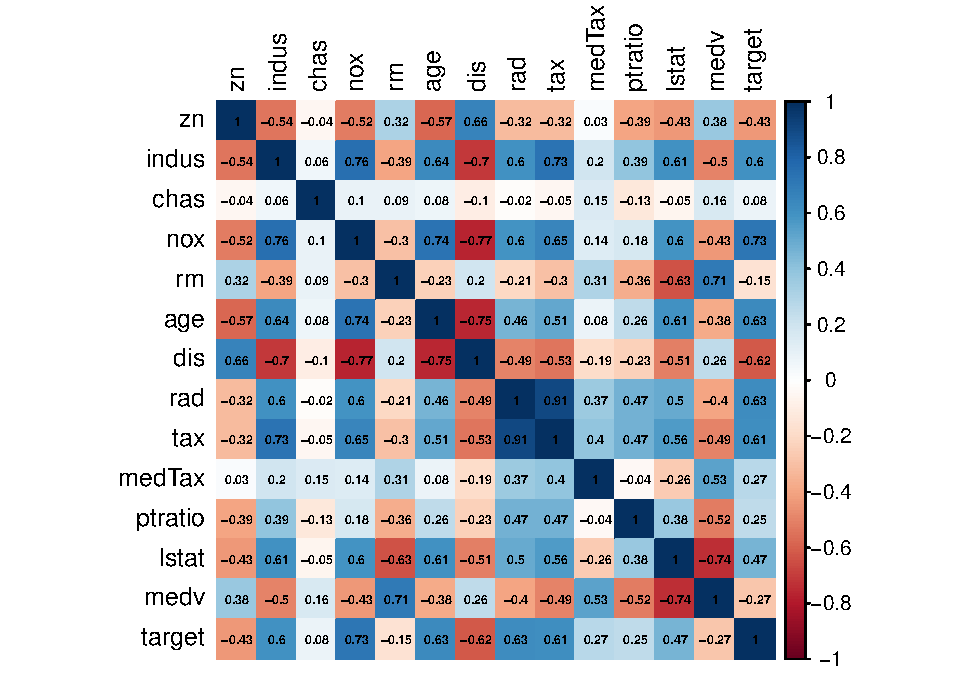
\includegraphics{NYCRealEstate_files/figure-latex/unnamed-chunk-12-1.pdf}

\begin{Shaded}
\begin{Highlighting}[]
\FunctionTok{str}\NormalTok{(clean\_nyc)}
\end{Highlighting}
\end{Shaded}

\begin{verbatim}
## 'data.frame':    1149281 obs. of  21 variables:
##  $ BOROUGH                       : int  1 1 1 1 1 1 1 1 1 1 ...
##  $ NEIGHBORHOOD                  : chr  "ALPHABET CITY" "CHELSEA" "CHELSEA" "CLINTON" ...
##  $ BUILDING.CLASS.CATEGORY       : Factor w/ 124 levels "                                            ",..: 4 4 12 12 8 4 4 4 8 8 ...
##  $ TAX.CLASS.AT.PRESENT          : Factor w/ 11 levels " ","  ","1","1A",..: 3 3 3 3 3 3 3 3 3 3 ...
##  $ BLOCK                         : int  374 722 772 1056 467 573 630 640 587 592 ...
##  $ LOT                           : int  46 72 42 24 52 59 2 70 64 11 ...
##  $ EASE.MENT                     : chr  "" "" "" "" ...
##  $ BUILDING.CLASS.AT.PRESENT     : Factor w/ 129 levels " ","  ","A0",..: 7 12 17 17 16 12 7 12 16 13 ...
##  $ ADDRESS                       : chr  "347 EAST 4TH STREET" "460 WEST 25TH STREET" "205 WEST 22ND STREET" "417 WEST 46TH STREET" ...
##  $ APARTMENT.NUMBER              : chr  "" "" "" "" ...
##  $ ZIP.CODE                      : num  10009 10001 10011 10036 10003 ...
##  $ RESIDENTIAL.UNITS             : num  1 1 3 3 2 1 1 1 2 2 ...
##  $ TOTAL.UNITS                   : num  1 1 3 3 2 1 1 1 2 2 ...
##  $ LAND.SQUARE.FEET              : num  2116 1626 822 2007 1700 ...
##  $ GROSS.SQUARE.FEET             : num  4400 3721 2776 4304 3740 ...
##  $ YEAR.BUILT                    : num  1900 1910 1901 1901 1899 ...
##  $ TAX.CLASS.AT.TIME.OF.SALE     : Factor w/ 4 levels "1","2","3","4": 1 1 1 1 1 1 1 1 1 1 ...
##  $ BUILDING.CLASS.AT.TIME.OF.SALE: chr  "A4" "A9" "C0" "C0" ...
##  $ SALE.PRICE                    : num  399000 0 0 0 0 0 0 0 0 0 ...
##  $ SALE.DATE                     : chr  "2022-09-29 00:00:00" "2022-03-10 00:00:00" "2022-02-10 00:00:00" "2022-07-20 00:00:00" ...
##  $ SALE_DATE                     : Date, format: "2022-09-29" "2022-03-10" ...
\end{verbatim}

\hypertarget{key-factors-influencing-real-estate-prices}{%
\subsubsection{Key Factors Influencing Real Estate
Prices}\label{key-factors-influencing-real-estate-prices}}

The linear regression model suggests that various factors significantly
influence real estate prices in New York City. Notably, residential
units, tax class, year built, sale date, tax class at time of sale,
gross square feet, and land square feet all demonstrate statistically
significant relationships with sale prices. However, the model's
adjusted R-squared value of 0.06164 indicates that only about 6.164\% of
the variability in sale prices is explained by these factors.
Additionally, the residuals' distribution reveals a considerable spread,
indicating potential heteroscedasticity or unaccounted-for factors in
the model.

\begin{Shaded}
\begin{Highlighting}[]
\CommentTok{\# regression analysis}
\NormalTok{lm\_model }\OtherTok{\textless{}{-}} \FunctionTok{lm}\NormalTok{(SALE.PRICE }\SpecialCharTok{\textasciitilde{}}\NormalTok{ RESIDENTIAL.UNITS }\SpecialCharTok{+}\NormalTok{ TAX.CLASS.AT.PRESENT }\SpecialCharTok{+}\NormalTok{ YEAR.BUILT }\SpecialCharTok{+}\NormalTok{ SALE\_DATE }\SpecialCharTok{+}\NormalTok{ TAX.CLASS.AT.TIME.OF.SALE }\SpecialCharTok{+}\NormalTok{ GROSS.SQUARE.FEET }\SpecialCharTok{+}\NormalTok{ LAND.SQUARE.FEET, }\AttributeTok{data =}\NormalTok{ clean\_nyc)}
\FunctionTok{summary}\NormalTok{(lm\_model)}
\end{Highlighting}
\end{Shaded}

\begin{verbatim}
## 
## Call:
## lm(formula = SALE.PRICE ~ RESIDENTIAL.UNITS + TAX.CLASS.AT.PRESENT + 
##     YEAR.BUILT + SALE_DATE + TAX.CLASS.AT.TIME.OF.SALE + GROSS.SQUARE.FEET + 
##     LAND.SQUARE.FEET, data = clean_nyc)
## 
## Residuals:
##     Min      1Q  Median      3Q     Max 
## -775674 -321371  -42793  227956 1621763 
## 
## Coefficients:
##                                Estimate   Std. Error t value
## (Intercept)                 233521.3963   11343.9261  20.586
## RESIDENTIAL.UNITS            39787.3198     706.6867  56.301
## TAX.CLASS.AT.PRESENT       -204939.9079   10595.8855 -19.341
## TAX.CLASS.AT.PRESENT1      -332391.9904   11120.0074 -29.891
## TAX.CLASS.AT.PRESENT1A     -267384.5810   11232.6810 -23.804
## TAX.CLASS.AT.PRESENT1B     -429788.1121   11315.1214 -37.984
## TAX.CLASS.AT.PRESENT1C     -103921.4024   13997.6874  -7.424
## TAX.CLASS.AT.PRESENT1D     -218870.2787   24130.4554  -9.070
## TAX.CLASS.AT.PRESENT2      -193655.0806    9870.1175 -19.620
## TAX.CLASS.AT.PRESENT2C     -102191.1926   10150.2536 -10.068
## TAX.CLASS.AT.PRESENT3      -407329.4338  136065.8992  -2.994
## TAX.CLASS.AT.PRESENT4      -314626.6682   11079.0815 -28.398
## YEAR.BUILT                       5.4097       0.7650   7.071
## SALE_DATE                       18.6537       0.1876  99.407
## TAX.CLASS.AT.TIME.OF.SALE2  102950.7101    6465.4286  15.923
## TAX.CLASS.AT.TIME.OF.SALE3  -63295.0519  130266.4276  -0.486
## TAX.CLASS.AT.TIME.OF.SALE4 -163815.1670    5939.8191 -27.579
## GROSS.SQUARE.FEET               13.8087       0.6852  20.154
## LAND.SQUARE.FEET                19.2470       0.3839  50.138
##                                        Pr(>|t|)    
## (Intercept)                < 0.0000000000000002 ***
## RESIDENTIAL.UNITS          < 0.0000000000000002 ***
## TAX.CLASS.AT.PRESENT       < 0.0000000000000002 ***
## TAX.CLASS.AT.PRESENT1      < 0.0000000000000002 ***
## TAX.CLASS.AT.PRESENT1A     < 0.0000000000000002 ***
## TAX.CLASS.AT.PRESENT1B     < 0.0000000000000002 ***
## TAX.CLASS.AT.PRESENT1C        0.000000000000114 ***
## TAX.CLASS.AT.PRESENT1D     < 0.0000000000000002 ***
## TAX.CLASS.AT.PRESENT2      < 0.0000000000000002 ***
## TAX.CLASS.AT.PRESENT2C     < 0.0000000000000002 ***
## TAX.CLASS.AT.PRESENT3                   0.00276 ** 
## TAX.CLASS.AT.PRESENT4      < 0.0000000000000002 ***
## YEAR.BUILT                    0.000000000001536 ***
## SALE_DATE                  < 0.0000000000000002 ***
## TAX.CLASS.AT.TIME.OF.SALE2 < 0.0000000000000002 ***
## TAX.CLASS.AT.TIME.OF.SALE3              0.62705    
## TAX.CLASS.AT.TIME.OF.SALE4 < 0.0000000000000002 ***
## GROSS.SQUARE.FEET          < 0.0000000000000002 ***
## LAND.SQUARE.FEET           < 0.0000000000000002 ***
## ---
## Signif. codes:  0 '***' 0.001 '**' 0.01 '*' 0.05 '.' 0.1 ' ' 1
## 
## Residual standard error: 367900 on 1149262 degrees of freedom
## Multiple R-squared:  0.06165,    Adjusted R-squared:  0.06164 
## F-statistic:  4195 on 18 and 1149262 DF,  p-value: < 0.00000000000000022
\end{verbatim}

The stepwise regression process, with a starting AIC of 29457675,
selected a final model with predictors including residential units, tax
class, year built, sale date, tax class at the time of sale, gross
square feet, and land square feet. This model, fitted using linear
regression, reveals statistically significant relationships between
these predictors and sale prices, as indicated by the low p-values and
the coefficients' significance levels. However, the adjusted R-squared
value remains low at 0.06164, suggesting that this model explains only a
small portion of the variability in sale prices.

\begin{Shaded}
\begin{Highlighting}[]
\CommentTok{\# Perform stepwise regression}
\NormalTok{stepwise\_model }\OtherTok{\textless{}{-}} \FunctionTok{step}\NormalTok{(lm\_model)}
\end{Highlighting}
\end{Shaded}

\begin{verbatim}
## Start:  AIC=29457675
## SALE.PRICE ~ RESIDENTIAL.UNITS + TAX.CLASS.AT.PRESENT + YEAR.BUILT + 
##     SALE_DATE + TAX.CLASS.AT.TIME.OF.SALE + GROSS.SQUARE.FEET + 
##     LAND.SQUARE.FEET
## 
##                             Df        Sum of Sq                RSS      AIC
## <none>                                          155591315571405088 29457675
## - YEAR.BUILT                 1    6769530540384 155598085101945472 29457723
## - GROSS.SQUARE.FEET          1   54990716199232 155646306287604320 29458080
## - TAX.CLASS.AT.TIME.OF.SALE  3  197247391038944 155788562962444032 29459126
## - LAND.SQUARE.FEET           1  340328837159072 155931644408564160 29460185
## - RESIDENTIAL.UNITS          1  429142788856672 156020458360261760 29460839
## - TAX.CLASS.AT.PRESENT      10  658928982669696 156250244554074784 29462512
## - SALE_DATE                  1 1337840771901312 156929156343306400 29467513
\end{verbatim}

\begin{Shaded}
\begin{Highlighting}[]
\CommentTok{\# Summary of the stepwise model}
\FunctionTok{summary}\NormalTok{(stepwise\_model)}
\end{Highlighting}
\end{Shaded}

\begin{verbatim}
## 
## Call:
## lm(formula = SALE.PRICE ~ RESIDENTIAL.UNITS + TAX.CLASS.AT.PRESENT + 
##     YEAR.BUILT + SALE_DATE + TAX.CLASS.AT.TIME.OF.SALE + GROSS.SQUARE.FEET + 
##     LAND.SQUARE.FEET, data = clean_nyc)
## 
## Residuals:
##     Min      1Q  Median      3Q     Max 
## -775674 -321371  -42793  227956 1621763 
## 
## Coefficients:
##                                Estimate   Std. Error t value
## (Intercept)                 233521.3963   11343.9261  20.586
## RESIDENTIAL.UNITS            39787.3198     706.6867  56.301
## TAX.CLASS.AT.PRESENT       -204939.9079   10595.8855 -19.341
## TAX.CLASS.AT.PRESENT1      -332391.9904   11120.0074 -29.891
## TAX.CLASS.AT.PRESENT1A     -267384.5810   11232.6810 -23.804
## TAX.CLASS.AT.PRESENT1B     -429788.1121   11315.1214 -37.984
## TAX.CLASS.AT.PRESENT1C     -103921.4024   13997.6874  -7.424
## TAX.CLASS.AT.PRESENT1D     -218870.2787   24130.4554  -9.070
## TAX.CLASS.AT.PRESENT2      -193655.0806    9870.1175 -19.620
## TAX.CLASS.AT.PRESENT2C     -102191.1926   10150.2536 -10.068
## TAX.CLASS.AT.PRESENT3      -407329.4338  136065.8992  -2.994
## TAX.CLASS.AT.PRESENT4      -314626.6682   11079.0815 -28.398
## YEAR.BUILT                       5.4097       0.7650   7.071
## SALE_DATE                       18.6537       0.1876  99.407
## TAX.CLASS.AT.TIME.OF.SALE2  102950.7101    6465.4286  15.923
## TAX.CLASS.AT.TIME.OF.SALE3  -63295.0519  130266.4276  -0.486
## TAX.CLASS.AT.TIME.OF.SALE4 -163815.1670    5939.8191 -27.579
## GROSS.SQUARE.FEET               13.8087       0.6852  20.154
## LAND.SQUARE.FEET                19.2470       0.3839  50.138
##                                        Pr(>|t|)    
## (Intercept)                < 0.0000000000000002 ***
## RESIDENTIAL.UNITS          < 0.0000000000000002 ***
## TAX.CLASS.AT.PRESENT       < 0.0000000000000002 ***
## TAX.CLASS.AT.PRESENT1      < 0.0000000000000002 ***
## TAX.CLASS.AT.PRESENT1A     < 0.0000000000000002 ***
## TAX.CLASS.AT.PRESENT1B     < 0.0000000000000002 ***
## TAX.CLASS.AT.PRESENT1C        0.000000000000114 ***
## TAX.CLASS.AT.PRESENT1D     < 0.0000000000000002 ***
## TAX.CLASS.AT.PRESENT2      < 0.0000000000000002 ***
## TAX.CLASS.AT.PRESENT2C     < 0.0000000000000002 ***
## TAX.CLASS.AT.PRESENT3                   0.00276 ** 
## TAX.CLASS.AT.PRESENT4      < 0.0000000000000002 ***
## YEAR.BUILT                    0.000000000001536 ***
## SALE_DATE                  < 0.0000000000000002 ***
## TAX.CLASS.AT.TIME.OF.SALE2 < 0.0000000000000002 ***
## TAX.CLASS.AT.TIME.OF.SALE3              0.62705    
## TAX.CLASS.AT.TIME.OF.SALE4 < 0.0000000000000002 ***
## GROSS.SQUARE.FEET          < 0.0000000000000002 ***
## LAND.SQUARE.FEET           < 0.0000000000000002 ***
## ---
## Signif. codes:  0 '***' 0.001 '**' 0.01 '*' 0.05 '.' 0.1 ' ' 1
## 
## Residual standard error: 367900 on 1149262 degrees of freedom
## Multiple R-squared:  0.06165,    Adjusted R-squared:  0.06164 
## F-statistic:  4195 on 18 and 1149262 DF,  p-value: < 0.00000000000000022
\end{verbatim}

Considering that Normality was not satisfied

The next model fitted using generalized linear regression with a
Gaussian family and an identity link function maintains predictors
including residential units, tax class, year built, sale date, tax class
at the time of sale, gross square feet, and land square feet. The
coefficients and their significance remain consistent with the previous
models. The null and residual deviances provide additional information
on the goodness of fit, with the residual deviance being slightly lower
than the null deviance, suggesting some level of model improvement.

\begin{Shaded}
\begin{Highlighting}[]
\CommentTok{\# Fit GLM with different error distribution and link function}
\NormalTok{glm\_model }\OtherTok{\textless{}{-}} \FunctionTok{glm}\NormalTok{(SALE.PRICE }\SpecialCharTok{\textasciitilde{}}\NormalTok{ RESIDENTIAL.UNITS }\SpecialCharTok{+}\NormalTok{ TAX.CLASS.AT.PRESENT }\SpecialCharTok{+}\NormalTok{ YEAR.BUILT }\SpecialCharTok{+}\NormalTok{ SALE\_DATE }\SpecialCharTok{+}\NormalTok{ TAX.CLASS.AT.TIME.OF.SALE }\SpecialCharTok{+}\NormalTok{ GROSS.SQUARE.FEET }\SpecialCharTok{+}\NormalTok{ LAND.SQUARE.FEET, }
                 \AttributeTok{data =}\NormalTok{ clean\_nyc, }
                 \AttributeTok{family =} \FunctionTok{gaussian}\NormalTok{(}\AttributeTok{link =} \StringTok{"identity"}\NormalTok{))}
\FunctionTok{summary}\NormalTok{(glm\_model)}
\end{Highlighting}
\end{Shaded}

\begin{verbatim}
## 
## Call:
## glm(formula = SALE.PRICE ~ RESIDENTIAL.UNITS + TAX.CLASS.AT.PRESENT + 
##     YEAR.BUILT + SALE_DATE + TAX.CLASS.AT.TIME.OF.SALE + GROSS.SQUARE.FEET + 
##     LAND.SQUARE.FEET, family = gaussian(link = "identity"), data = clean_nyc)
## 
## Coefficients:
##                                Estimate   Std. Error t value
## (Intercept)                 233521.3963   11343.9261  20.586
## RESIDENTIAL.UNITS            39787.3198     706.6867  56.301
## TAX.CLASS.AT.PRESENT       -204939.9079   10595.8855 -19.341
## TAX.CLASS.AT.PRESENT1      -332391.9904   11120.0074 -29.891
## TAX.CLASS.AT.PRESENT1A     -267384.5810   11232.6810 -23.804
## TAX.CLASS.AT.PRESENT1B     -429788.1121   11315.1214 -37.984
## TAX.CLASS.AT.PRESENT1C     -103921.4024   13997.6874  -7.424
## TAX.CLASS.AT.PRESENT1D     -218870.2787   24130.4554  -9.070
## TAX.CLASS.AT.PRESENT2      -193655.0806    9870.1175 -19.620
## TAX.CLASS.AT.PRESENT2C     -102191.1926   10150.2536 -10.068
## TAX.CLASS.AT.PRESENT3      -407329.4338  136065.8992  -2.994
## TAX.CLASS.AT.PRESENT4      -314626.6682   11079.0815 -28.398
## YEAR.BUILT                       5.4097       0.7650   7.071
## SALE_DATE                       18.6537       0.1876  99.407
## TAX.CLASS.AT.TIME.OF.SALE2  102950.7101    6465.4286  15.923
## TAX.CLASS.AT.TIME.OF.SALE3  -63295.0519  130266.4276  -0.486
## TAX.CLASS.AT.TIME.OF.SALE4 -163815.1670    5939.8191 -27.579
## GROSS.SQUARE.FEET               13.8087       0.6852  20.154
## LAND.SQUARE.FEET                19.2470       0.3839  50.138
##                                        Pr(>|t|)    
## (Intercept)                < 0.0000000000000002 ***
## RESIDENTIAL.UNITS          < 0.0000000000000002 ***
## TAX.CLASS.AT.PRESENT       < 0.0000000000000002 ***
## TAX.CLASS.AT.PRESENT1      < 0.0000000000000002 ***
## TAX.CLASS.AT.PRESENT1A     < 0.0000000000000002 ***
## TAX.CLASS.AT.PRESENT1B     < 0.0000000000000002 ***
## TAX.CLASS.AT.PRESENT1C        0.000000000000114 ***
## TAX.CLASS.AT.PRESENT1D     < 0.0000000000000002 ***
## TAX.CLASS.AT.PRESENT2      < 0.0000000000000002 ***
## TAX.CLASS.AT.PRESENT2C     < 0.0000000000000002 ***
## TAX.CLASS.AT.PRESENT3                   0.00276 ** 
## TAX.CLASS.AT.PRESENT4      < 0.0000000000000002 ***
## YEAR.BUILT                    0.000000000001536 ***
## SALE_DATE                  < 0.0000000000000002 ***
## TAX.CLASS.AT.TIME.OF.SALE2 < 0.0000000000000002 ***
## TAX.CLASS.AT.TIME.OF.SALE3              0.62705    
## TAX.CLASS.AT.TIME.OF.SALE4 < 0.0000000000000002 ***
## GROSS.SQUARE.FEET          < 0.0000000000000002 ***
## LAND.SQUARE.FEET           < 0.0000000000000002 ***
## ---
## Signif. codes:  0 '***' 0.001 '**' 0.01 '*' 0.05 '.' 0.1 ' ' 1
## 
## (Dispersion parameter for gaussian family taken to be 135383677152)
## 
##     Null deviance: 165814015036012544  on 1149280  degrees of freedom
## Residual deviance: 155591315571405312  on 1149262  degrees of freedom
## AIC: 32719196
## 
## Number of Fisher Scoring iterations: 2
\end{verbatim}

The final model, fitted using robust linear regression (rlm), estimates
the intercept at \$290,788.64. Each additional residential unit
increases the sale price by \$33,326.57. For the tax class at present,
each category shows significant negative impacts on the sale price, with
Tax Class 1B having the largest effect, reducing the price by
\$436,466.67. A one-unit increase in the year built is associated with a
\$9.05 increase in sale price. Similarly, each day increment in the sale
date adds \$14.35 to the sale price. Other variables, such as gross
square feet and land square feet, also exhibit significant positive
effects on the sale price. The residual standard error, indicating the
model's accuracy, is \$428,200.

\begin{Shaded}
\begin{Highlighting}[]
\FunctionTok{library}\NormalTok{(MASS)}

\CommentTok{\# Fit robust linear regression model}
\NormalTok{lm\_model\_robust }\OtherTok{\textless{}{-}} \FunctionTok{rlm}\NormalTok{(SALE.PRICE }\SpecialCharTok{\textasciitilde{}}\NormalTok{ RESIDENTIAL.UNITS }\SpecialCharTok{+}\NormalTok{ TAX.CLASS.AT.PRESENT }\SpecialCharTok{+}\NormalTok{ YEAR.BUILT }\SpecialCharTok{+}\NormalTok{ SALE\_DATE }\SpecialCharTok{+}\NormalTok{ TAX.CLASS.AT.TIME.OF.SALE }\SpecialCharTok{+}\NormalTok{ GROSS.SQUARE.FEET }\SpecialCharTok{+}\NormalTok{ LAND.SQUARE.FEET, }
                       \AttributeTok{data =}\NormalTok{ clean\_nyc)}
\FunctionTok{summary}\NormalTok{(lm\_model\_robust)}
\end{Highlighting}
\end{Shaded}

\begin{verbatim}
## 
## Call: rlm(formula = SALE.PRICE ~ RESIDENTIAL.UNITS + TAX.CLASS.AT.PRESENT + 
##     YEAR.BUILT + SALE_DATE + TAX.CLASS.AT.TIME.OF.SALE + GROSS.SQUARE.FEET + 
##     LAND.SQUARE.FEET, data = clean_nyc)
## Residuals:
##     Min      1Q  Median      3Q     Max 
## -689412 -310434  -23950  245265 1635049 
## 
## Coefficients:
##                            Value        Std. Error   t value     
## (Intercept)                 290788.6415   10750.8300      27.0480
## RESIDENTIAL.UNITS            33326.5719     669.7389      49.7605
## TAX.CLASS.AT.PRESENT       -231264.0838   10041.8993     -23.0299
## TAX.CLASS.AT.PRESENT1      -311659.8313   10538.6185     -29.5731
## TAX.CLASS.AT.PRESENT1A     -260618.5149   10645.4012     -24.4818
## TAX.CLASS.AT.PRESENT1B     -436466.6668   10723.5312     -40.7018
## TAX.CLASS.AT.PRESENT1C     -137901.4600   13265.8443     -10.3952
## TAX.CLASS.AT.PRESENT1D     -210361.9947   22868.8393      -9.1986
## TAX.CLASS.AT.PRESENT2      -211613.8859    9354.0768     -22.6226
## TAX.CLASS.AT.PRESENT2C     -112557.9271    9619.5664     -11.7009
## TAX.CLASS.AT.PRESENT3      -416669.1176  128951.9462      -3.2312
## TAX.CLASS.AT.PRESENT4      -316231.0765   10499.8323     -30.1177
## YEAR.BUILT                       9.0531       0.7250      12.4866
## SALE_DATE                       14.3494       0.1778      80.6878
## TAX.CLASS.AT.TIME.OF.SALE2   93751.7630    6127.3957      15.3004
## TAX.CLASS.AT.TIME.OF.SALE3  -49322.2028  123455.6892      -0.3995
## TAX.CLASS.AT.TIME.OF.SALE4 -168030.0667    5629.2667     -29.8494
## GROSS.SQUARE.FEET                5.3647       0.6493       8.2618
## LAND.SQUARE.FEET                18.0511       0.3638      49.6167
## 
## Residual standard error: 428200 on 1149262 degrees of freedom
\end{verbatim}

\end{document}
